% At the risk of making this even longer, you probably need a section on the optimization.  No more than a page, max...
\section{Neutron Interactions with Matter}

Neutron interaction mechanisms with matter serve as a physical constraint to spectral shaping of a neutron flux spectrum. 
Neutron interactions can act to moderate, absorb, or even emit more neutrons. 
The major reaction mechanisms available in the range of the fast to thermal energies that are relevant to nuclear weapon environments are elastic scattering, inelastic scattering, radiative capture, and the release of `x' particle (n,xn) reactions. 
Fission reactions are an extremely important reaction mechanism for the formation of synthetic weapon debris; however, fission does not contribute largely to the spectral modification problem for this application. 
A diagram summarizing the important neutron reactions is shown in Figure \ref{fig:rxns}.

\begin{figure}[ht]
	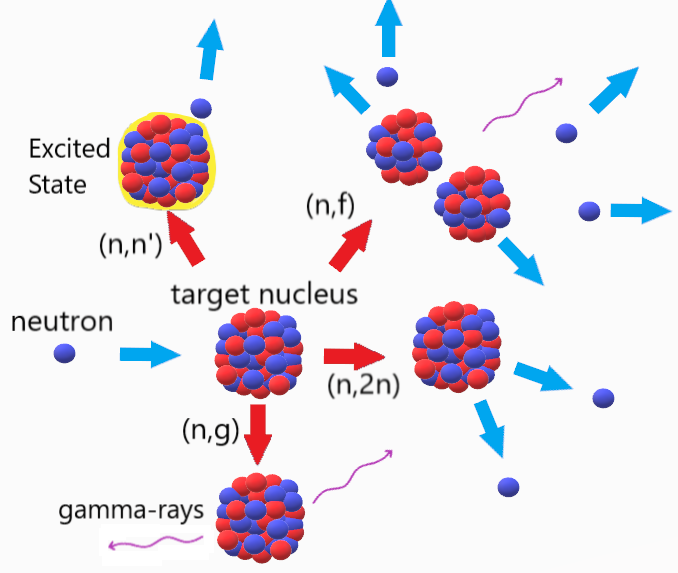
\includegraphics[width=\linewidth]{Figures/Chapter2/NeutronThings.png}
	\caption[Diagram of selected neutron reactions]{Diagram of selected neutron reactions important to various aspects of this work \cite{Greenwood2013}.}
	\label{fig:rxns}
\end{figure}

The neutron interaction probability is described by the neutron microscopic reaction cross-section ($\sigma_{rx}$), which is a function of the target isotope and incident neutron energy $(E_{n})$.  
The microscopic cross-section multiplied by the atomic number density, $N$, provides macroscopic cross-section ($\Sigma_{rx})$, a measure of the interaction probability in bulk material. 

Neutrons can be categorized into energy regimes such as thermal, epithermal, and fast, although these regions are relative and vary according to different fields of nuclear sciences or particle physics.  
A thermal neutron is below 0.025 eV, which is average neutron energy, ($E_{n}$), in thermal equilibrium with a 290 K temperature distribution\cite{Duderstadt}. 
Epithermal neutrons are between 0.025 eV and 1 MeV, and fast neutrons are above 1 MeV.
In this context of presenting fission product distributions as a function of energy, fast neutrons are a Watt spectrum at 500 keV, and high energy neutrons are 14 MeV. 

% Need a sentence to preface why the following section is here. As stated, it is unclear what value this para and figure add. I think I'll leave it off. 

%The major cross-sections of interest to $^{235}$U up to 20 MeV are displayed in Figure \ref{fig:ntotU}. 
%The total cross-section is the summation of all of the possible reaction mechanisms. 
%Each reaction is explained in further detail below; however, it is important to understand that these reactions are in competition with each other. 
%In general, absorption reactions dominate at low energy. 
%At high energy elastic scattering, inelastic scattering, and (n,xn) reactions are the most probable interaction. 

%\begin{figure}[ht]
%	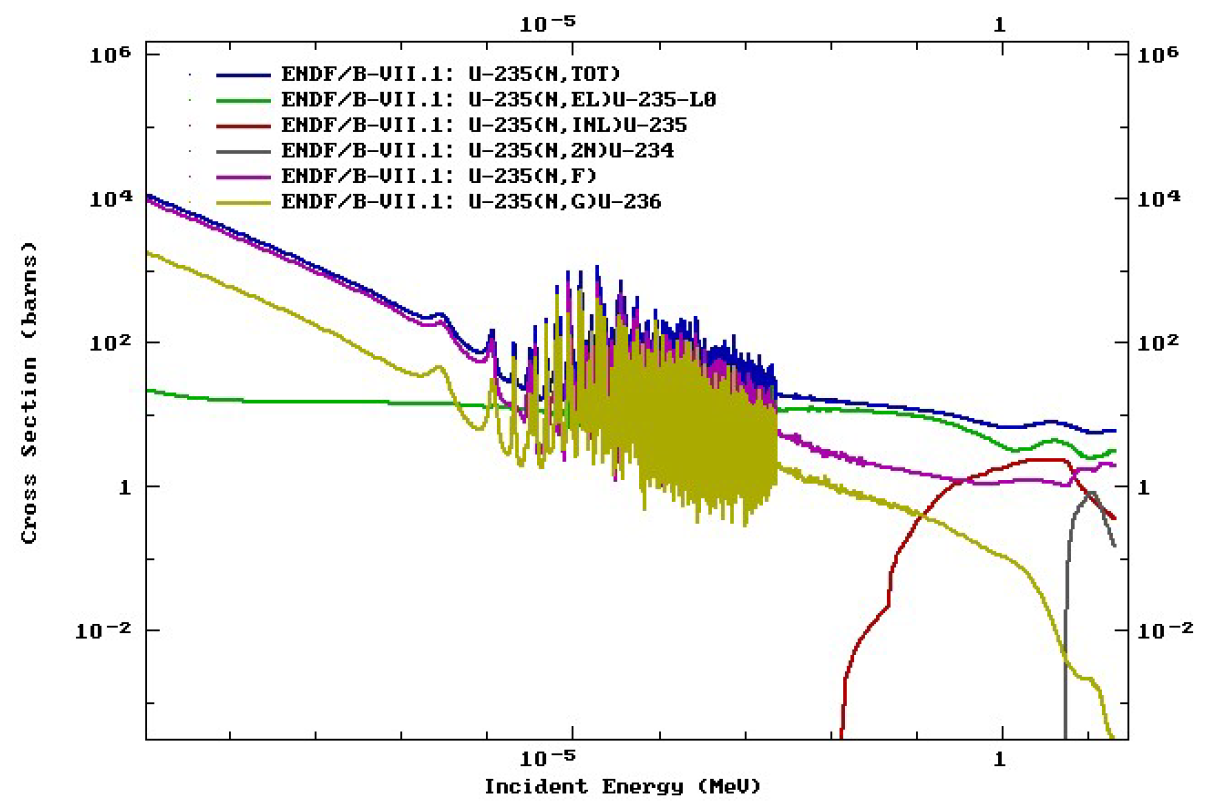
\includegraphics[width=\linewidth]{Figures/Chapter2/n_tot.png}
%	\caption[U-235 (n,f) cross-section compared to competing reaction channels]{U-235 (n,f) cross-section compared to competing reaction channels\cite{ENDF}}
%	\label{fig:ntotU}	
%\end{figure}

\subsection{n,n}

\ Elastic scattering (n,n) is an extremely important reaction for lowering the average energy of the neutron population by downscattering \cite{Turner}. 
An elastic collision does not place the target nucleus in an excited state, which allows for the simplified use of conservation of energy and momentum to describe the interaction. 
A selected group of elastic scattering cross-sections relevant to the application in an ETA are shown in Figure \ref{fig:elastic}. 

\begin{figure}[ht]
	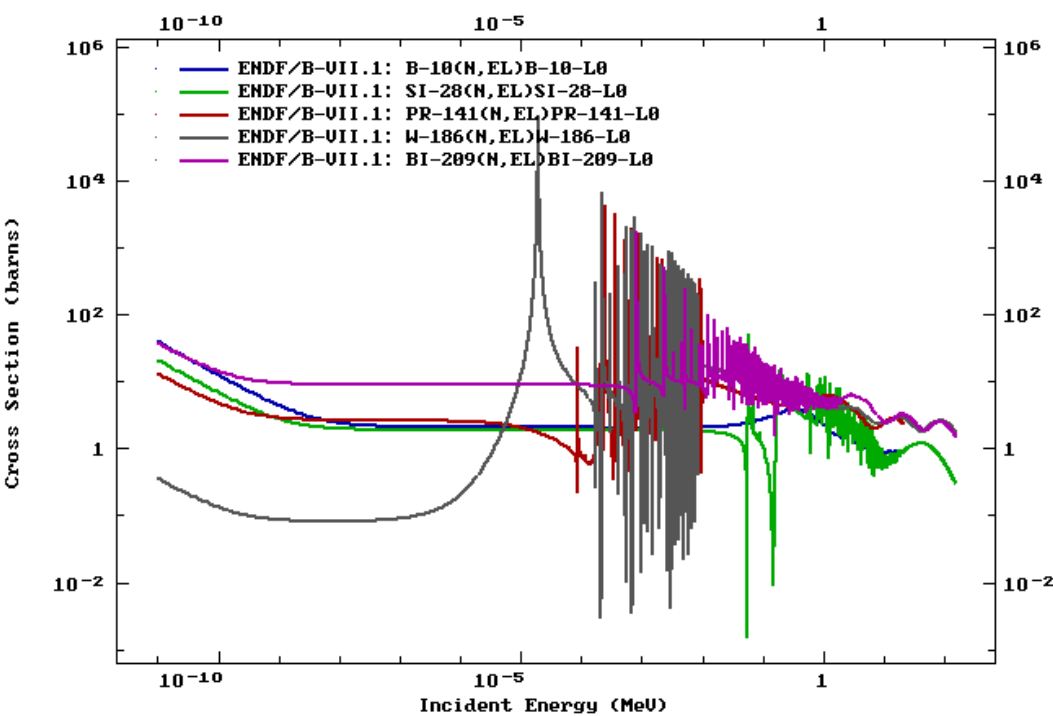
\includegraphics[width=\linewidth]{Figures/Chapter2/elastic.png}
	\caption[Comparison of various elastic scattering cross-sections for materials in the current ETA]{Comparison of various elastic scattering cross-sections for materials in the current ETA \cite{ENDF}.}
	\label{fig:elastic}
\end{figure}

\ The maximum energy lost in a neutron elastic collision with an isotope is a function of the target isotope atomic mass (M). 
Elastic scatters off higher mass isotopes produce a smaller energy loss per collision compared to interactions with low atomic mass nuclei. 
Elastic scattering can transfer nearly all of a neutron's kinetic energy with a collision on hydrogen, while scattering off bismuth will produce very little energy loss. 
The maximum energy transfer (Q) to the target nucleus per collision is given by: 

\begin{equation} \label{eq:elastic}
    Q_{max}=\dfrac{4ME_{n}}{(M+1)^{2}}
\end{equation}

\subsection{n,n'}

\ Inelastic scattering is similar to the reaction dynamics of elastic scattering; however, the target nucleus is placed in an energetically excited state\cite{Turner}.
These excited states are governed by quantum mechanics and are unique to particular isotopes. 
Nuclear excited states akin to the electronic shell structure of atoms. Hydrogen for example can have infinite electron shells with decreasing shell energy differential up to the ionization energy of the electron. An incident photon can populate the electron into an excited states, but nuclear states have a limited number of discrete levels. Two nuclei can form a quasi-continuous spectrum during a compound reaction which gives rise to resonances\cite{Krane}. These resonances have a certain energy width created by states having a energy widths larger than the energy spacing of the states. 

\ Inelastic scattering is a threshold reaction, meaning an incident neutron must have a minimum amount of energy to enable the reaction channel. 
Additionally, neutrons generally lose more energy per collision if the interaction is inelastic on high Z isotopes. 
The energy that would normally be conserved in the collision is reduced in the conservation equations. 
Examples of inelastic scattering cross-sections are shown in Figure \ref{fig:inelastic}. Isotopes from $A=12$ to $209$ are shown to identify the trend of increasing mass number. 

% Why the different isotopes in each plot? Different aspects are important. 
\begin{figure}[ht]
	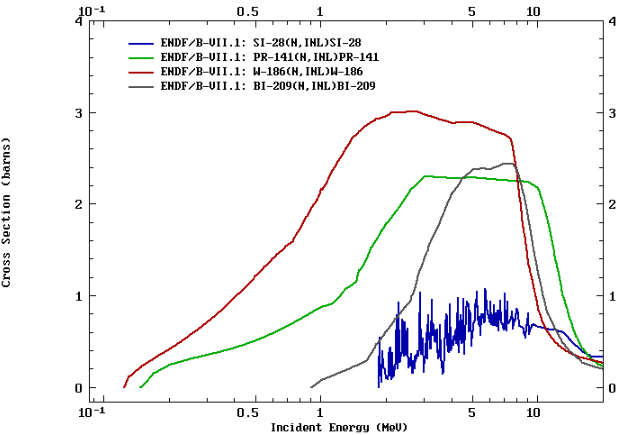
\includegraphics[width=\linewidth]{Figures/Chapter2/inelastic.png}
	\caption[Comparison of various inelastic scattering cross-sections for materials in the current ETA]{Comparison of various inelastic scattering cross-sections for materials in the current ETA\cite{ENDF}}
	\label{fig:inelastic}
\end{figure}

\ Inelastic scattering is one of the lowest threshold energy neutron reactions.
As shown in Figure \ref{fig:inelastic}, there is no general functional form of the reaction by isotope. 
Al-27, a lighter isotope, is between W-184 and Pb-208. 
These cross-sections indicate the energy levels of the nuclei itself. 
Threshold reactions are also of interest to determining the neutron spectrum for identifying the reaction rate above the threshold energy.

\ The excited state nucleus can de-excite via gamma emission or other channels if energetically favorable. 
The excited nucleus usually decays in a short time relative to isomeric states if the inelastic scatter occurs off of a stable nucleus. 
Isomers are not stable; however, these metastable states can have half-lives on the order of hours or much longer\cite{Krane}. 
These isomeric states have applications in foil activation experiments, where it may take some time to start measuring the foil activity. 
An energy level and decay mode diagram of In-116 is shown in Figure \ref{fig:In116Rxn}.
Depending on the selection rules, certain energy level transitions are available for a given neutron interaction \cite{Knoll}.  

\begin{figure}[ht]
	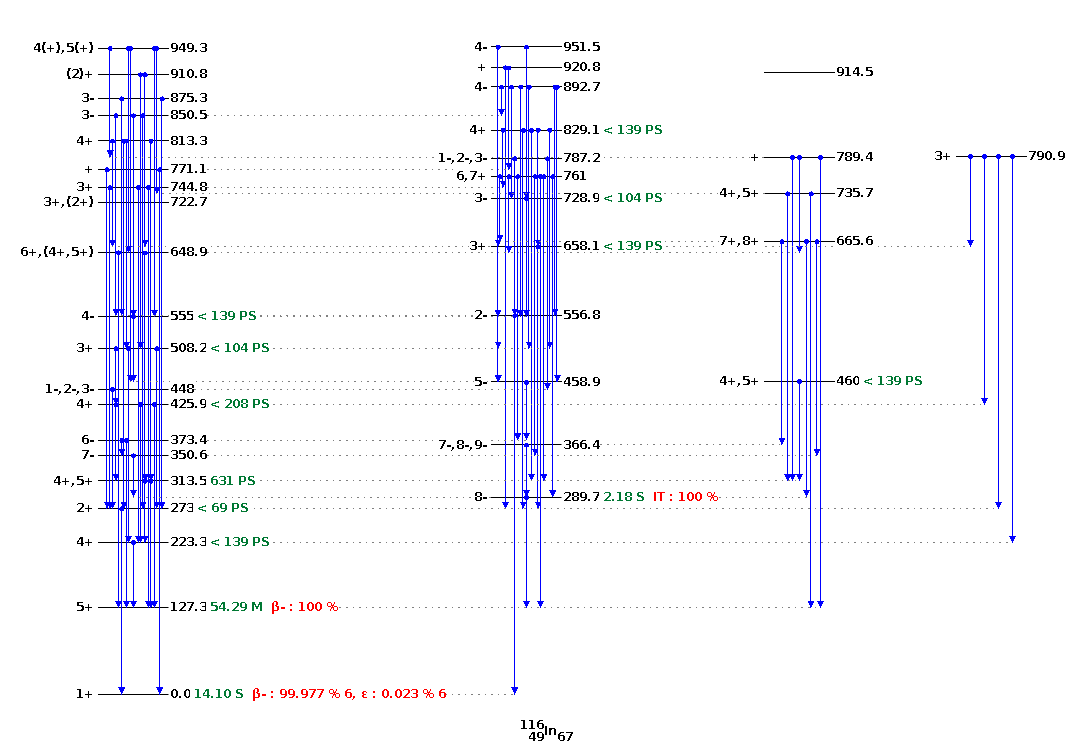
\includegraphics[width=\linewidth]{Figures/Chapter2/TruncatedIn116.png}
	\caption[In-116 energy level and decay mode diagram truncated at 970.4 keV]{In-116 energy level and decay mode diagram truncated at 970.4 keV. The metastable state at 127 keV with spin parity $J^{\pi} = 5^{+}$ is important for foil activation experiments for the epithermal region. Plots produced using the Online Service retrieval code package written by C. L. Dunford, National Nuclear Data Center, Brookhaven National Laboratory.}
	\label{fig:In116Rxn}
\end{figure}

\subsection{n,xn}

\ A neutron can interact with a nucleus and eject additional particles, such as neutrons or protons. 
(n,xn) reactions such as (n,2n) and (n,3n) require a threshold energy to separate the neutron from the original nucleus, appropriately called the neutron separation energy. 
Neutron separation energies are on the order of a few MeV to tens of MeV \cite{Krane,n2ns}. 
Increasing the neutron energy allows for the evaporation of more neutrons from the nucleus. 

\ The (n,xn) mechanism can occur as a direct reaction, where the incident proton interacts with only a few particles in the nucleus. 
Additionally, the neutron can interact with the entire nuclei and be absorbed in a resonance or compound reaction, later ejecting the particles \cite{Turner}. 
There is a large variance based on the internal nuclear structure. % Large variance in what?
Example (n,2n) reactions are shown in Figure \ref{fig:n2n}. 
The cross-section threshold is generally lower for higher atomic mass isotopes which are not as tightly bound to the neutron. 

\begin{figure}[ht]
	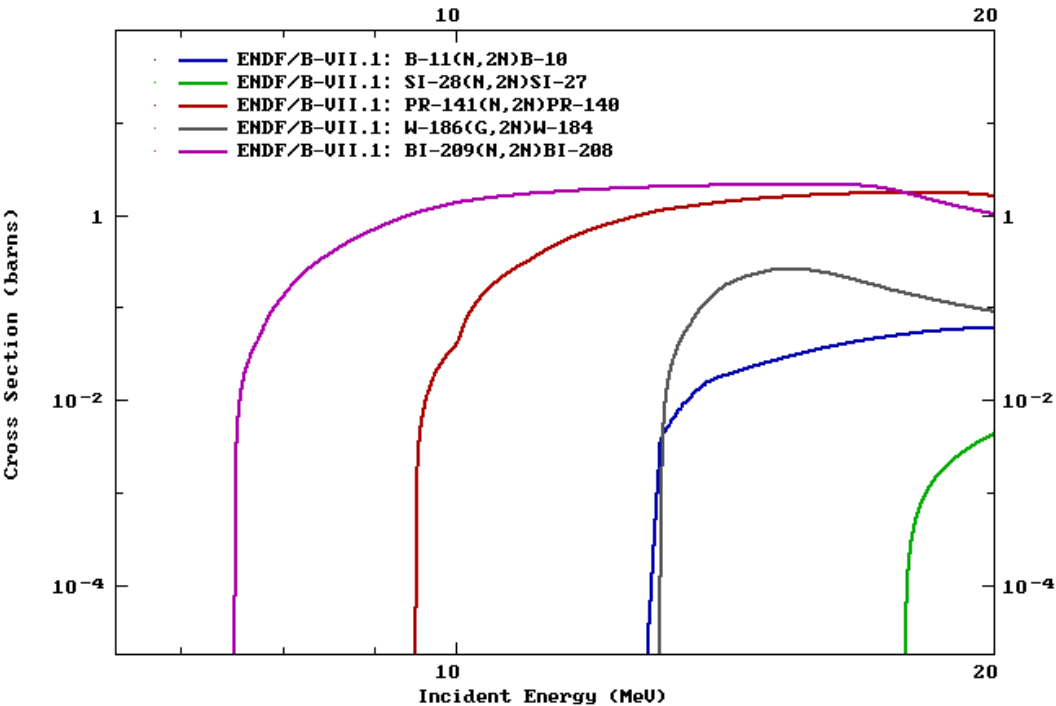
\includegraphics[width=\linewidth]{Figures/Chapter2/n2n.png}
	\caption[Comparison of various (n,2n) cross-sections for materials in the current ETA]{Comparison of various (n,2n) cross-sections for materials in the current ETA\cite{ENDF}}
	\label{fig:n2n}
\end{figure}

\ In the context of spectral shaping, (n,xn) reactions are significant for two reasons. 
First, the interaction increases the total neutron population which is beneficial for increasing the number of neutrons on the samples. 
Second, the neutron energy post-reaction is lower because the reaction required to overcome the potential barrier and losses through gamma emission. 
The lowered neutron energy is beneficial again for building up lower energy portions compared to the source term. 
Additionally, this reaction mechanism has applications in foil activation experiments.  

\subsection{n,$\gamma$}

Radiative capture, abeled (n,g) and (n,$\gamma$) in literature, is a reaction mechanism most prominent at low energies where an incident neutron is absorbed into the nucleus and a gamma-ray is emitted \cite{Krane}. 
%The gamma-rays emitted are important for determining the nuclear structure of the isotope. % This sentence seems irrelevant to this application.
At low energies (below approximatley 1 keV, isotope dependent) the absorption cross-section follows the ``1/v" law, so the probability increases with the inverse of the square of the incident neutron energy\cite{Turner}. 
Figure \ref{fig:ngamma} provides examples of selected (n,$\gamma$) cross-sections. 

\begin{figure}[ht]
	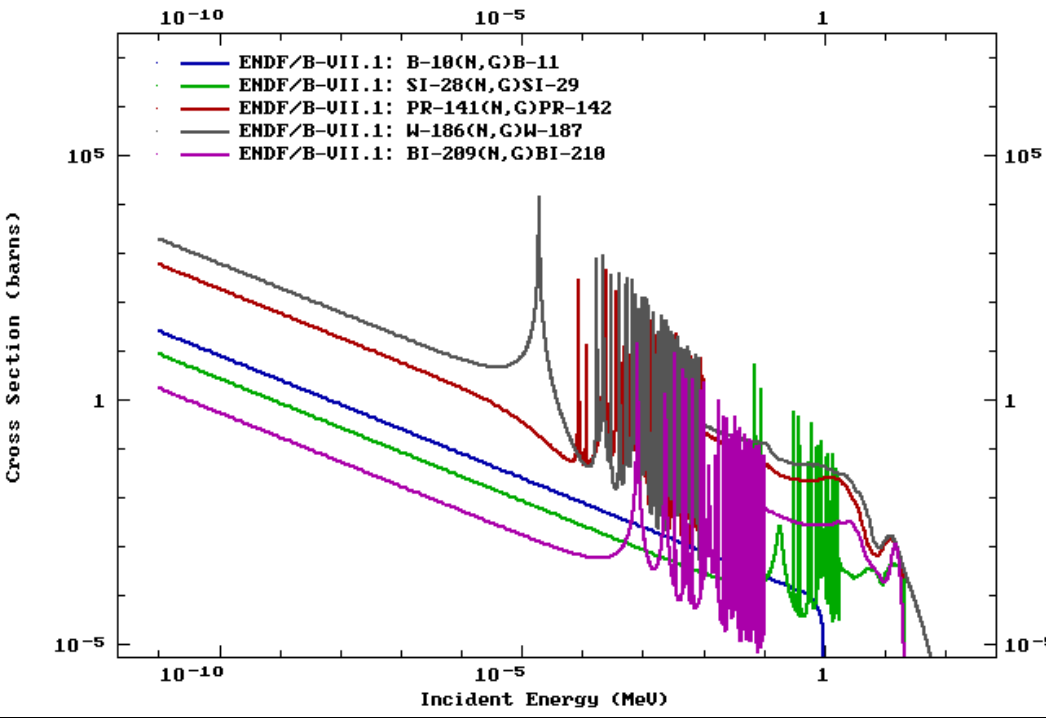
\includegraphics[width=\linewidth]{Figures/Chapter2/ngamma.png}
	\caption[Comparison of various (n,$\gamma$) cross-sections for materials in the current ETA]{Comparison of various (n,$\gamma$) cross-sections\cite{ENDF} for materials in the current ETA}
	\label{fig:ngamma}	
\end{figure}

\ Radiative capture is an important absorption reaction mechanism in a few ways. 
(n$\gamma$) reactions are of interest to foil activation experiments, specifically for determining the thermal spectrum. 
The resonance structure in the epithermal region can also be used to generate a unique response. 
Radiative capture is generally undesirable for spectral shaping, acting as a poison for the neutron economy. 
Fortunately, the NIF source, at 14 MeV, is not largely impacted until the neutrons have been moderated, but the ($n,\gamma$) reaction can be used to absorb an excess of thermal neutrons \cite{Bevins}. 

\section{Nuclear Fission}
\subsection{Fission Theory}
\ Nuclear fission reactions encompass the breakup of an unstable nucleus into two or more fission fragments. 
%An unstable compound nucleus formed from neutron induced fission can de-excite via radiative capture or fission. % Or neutron emission. Or proton. Or alpha. I'd delete 
Fission releases a large amount of energy (approximately 200 MeV), which is distributed as kinetic energy in the fission fragments, neutrons, gamma-rays, and delayed decay energy. 
The amount of energy liberated is dependent on the reaction products, so an average number is usually given.
The delayed portion is associated with the decay of the unstable fission fragments, which includes energy in the form of beta particles, additional gamma-rays, anti-neutrinos, and neutrons. 
A schematic of the fission process is shown in Figure \ref{fig:fission}.


\begin{figure}[ht]
	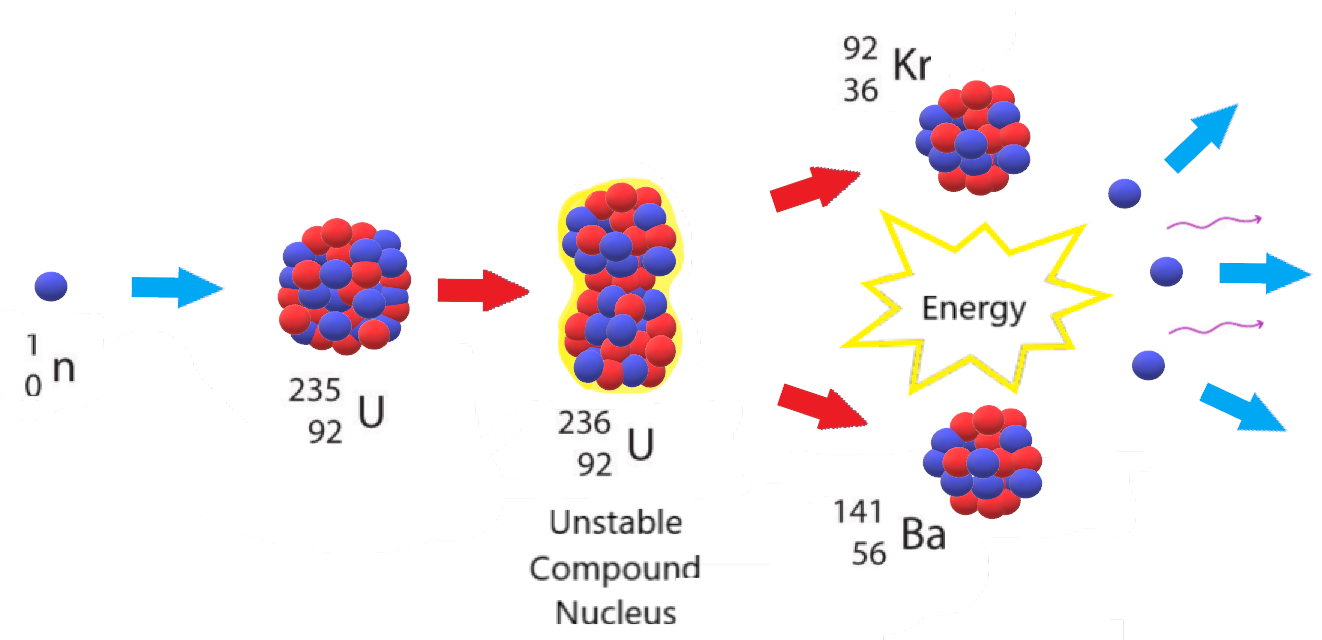
\includegraphics[width=\linewidth]{Figures/Chapter2/Fission.png}
	\caption{Schematic overview of $^{235}$U neutron induced fission. }
	\label{fig:fission}	
\end{figure}

Fission occurs most often in high atomic mass nuclei, such as $^{235}$U, $^{238}$U, or $^{239}$Pu; however, any isotope can be fissioned at large enough incident energies. 
The fissioned isotope separates into two or occasionally three nuclei\cite{Bridgman}. 
Fissionable isotopes, for example U-238, Pu-240, Pu-242, have a significant fission barrier, depressed fission cross-sections at low energy, and are incapable of sustaining a nuclear chain reaction. 
Fissile isotopes like U-235 and Pu-239 are capable of sustaining a nuclear chain reaction and have cross-sections with similar characteristics to the radiative capture cross-section. 

The unstable compound nucleus can be modeled at high neutron energies, well above the fission barrier, as an incompressible liquid drop\cite{Krane,Tonchev0}. 
The deformation of the nucleus causes increased surface energies, which are balanced with the Coulomb (charge repulsion), volume contribution, and shell pairing effects. 
The perturbation creates an increase to the surface energy and decrease of the Coulomb repulsion because the charge is spread out\cite{Randrup2012}. 
During the fission process, the evolving compound nucleus can emit pre-fission neutrons, known as multi-chance fission \cite{Randrup2012}. 
First-chance fission is the emission of no neutrons, second-chance fission is the emission of one neutron, and so on; % the use of \nu here is confusing as it normally refers to the total average neutrons emitted. I usually see that as nu_bar depending on what field. I see how that was confusing though. It didnt really add anything, so its gone. 
larger neutron energies are correlated with higher order chance fission. 
The average fission process releases 2-3 neutrons, and the average increases with incident neutron energy. 
The mean number of neutrons released per fission event is the neutron multiplicity.  

Immediately following the fission event, the fission fragments are at a highly excited state.
Fission fragments are generally very neutron rich compared to the valley of stability. 
The excited fragments emit photons to de-excite and may have enough energy to evaporate more neutrons \cite{Randrup2012}. 
The prompt fission product yield is the distribution of products post neutron evaporation from the fission fragments.  
% Inconsistent use of fragment vs product. I do not like the difference. The way I see it, the fission fragments come before the products. 

\subsection{Fission Products}

The fission product distribution from thermally induced fission tends to be centered around isotopes with closed nuclear shells. 
These isotopes are have a ``magic number" of protons and neutrons, similar to the filled electron structure of the noble gases. 
The fission fragment distribution of thermal neutrons incident on $^{235}$U is shown in Figure \ref{fig:GEF_U}. 

\begin{figure}[h!]
	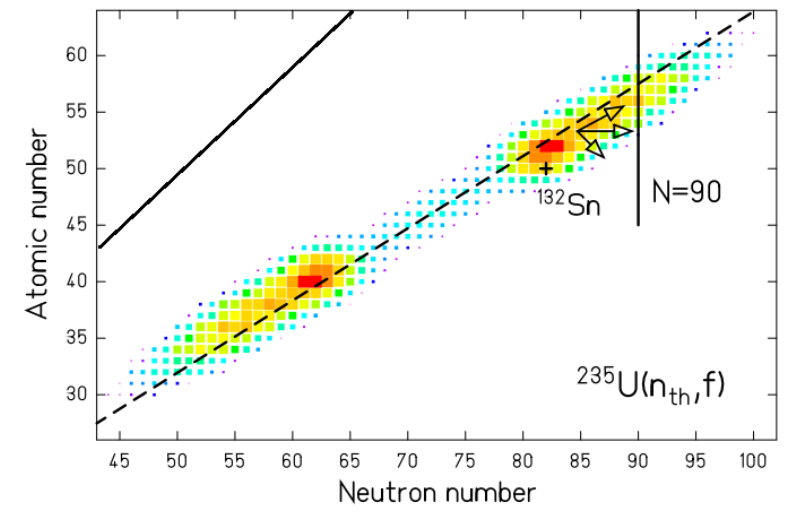
\includegraphics[width=\linewidth]{Figures/Chapter2/U_235Band.png}
	\caption[GEF calculated thermal fission product distribution prior to prompt neutron emission. The dashed line is the neutron to proton ratio of U-235 and the solid line is a neutron to proton ratio of 1]{GEF calculated thermal fission product distribution prior to prompt neutron emission. The dashed line is the neutron to proton ratio of U-235 and the solid line is a neutron to proton ratio of 1\cite{Schmidt2014}.}
	\label{fig:GEF_U}	
\end{figure}

Stable nuclei have approximately half as many protons to the total nucleons (neutrons and protons)\cite{Krane}. 
Larger nuclei require more neutrons to mitigate Coulomb repulsion. 
As noted, most of the decay processes following fission are beta emitters, which occurs because the products are rich in neutrons. 
Figure \ref{fig:DMode} shows the primary decay modes of isotopes as they decay to the valley of stability. 
In the region of fission products, the primary competing decay mode is neutron emission, resulting in mass chain feeding and loss after the initial fission process. 

\begin{figure}[h!]
	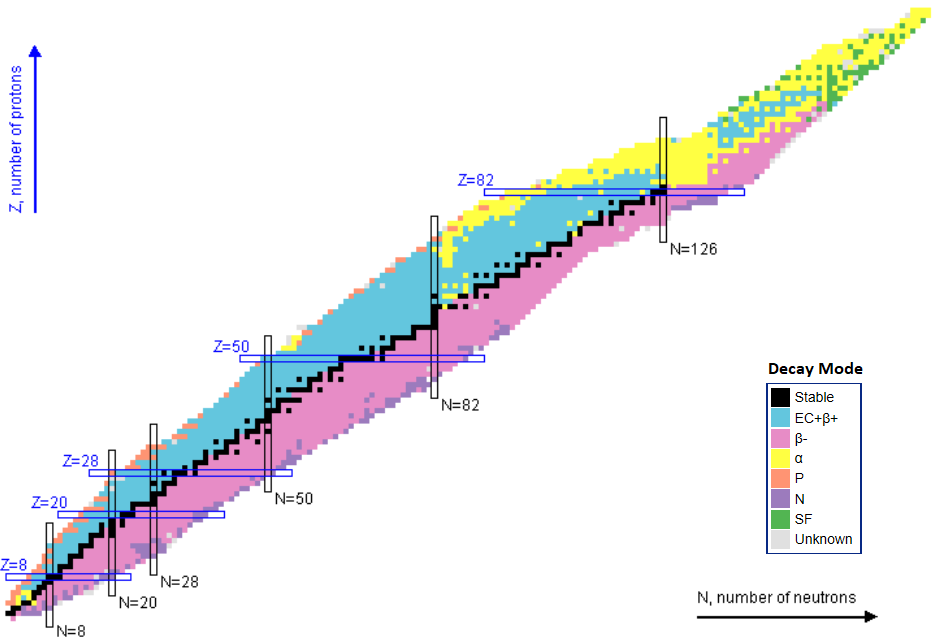
\includegraphics[width=\linewidth]{Figures/Chapter2/DecayModes.png}
	\caption[Primary decay modes of isotopes]{Primary decay modes of isotopes. Plots produced using the Online Service retrieval code package written by C. L. Dunford, National Nuclear Data Center, Brookhaven National Laboratory.}
	\label{fig:DMode}
\end{figure}

Fission yields can be described by the independent, cumulative, and chain yields\cite{Nichols2008}. % There has to be a better, original reference than me! This was too hard to find... it wasnt in any of my textbooks...
The independent yield,$Y_{ind}$, for thermal $^{235}$U fission is shown in Figure \ref{fig:indy} which is the fission products directly after the fission event before decay\cite{Nichols2008}. The fractional independent yield, $f(A,Z)$, defines the yield of a particular isotope. 
The sum yield, $Y(A)$, is the is the sum of all fission products for a given mass A. 
The isomeric yield ratio, $R(A,Z,I)$, is the the production of each isomer, $I$, for a given independent yield. 
The independent isomeric yield is defined as \cite{indy}

\begin{equation} \label{eq:Indy}
Y_{ind}(A,Z,I) = Y(A) \space f(A,Z) \space R(A,Z,I). 
\end{equation}

\begin{figure}[h!]
	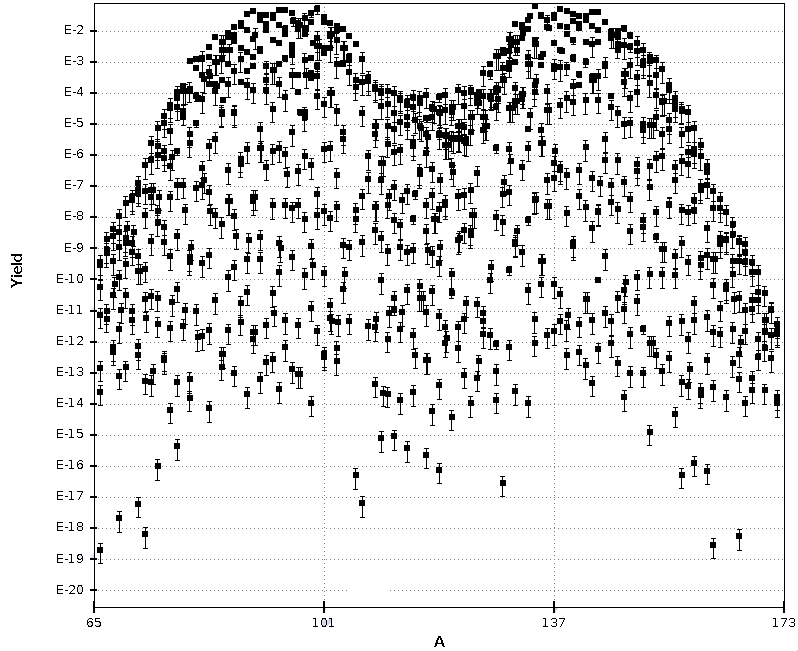
\includegraphics[width=\linewidth]{Figures/Chapter2/indfy.png}
	\caption[Independent fission product yield of thermal fission of U-235]{Independent fission product yield of thermal fission of U-235. Plots produced using the Online Service retrieval code package written by C. L. Dunford, National Nuclear Data Center, Brookhaven National Laboratory.}
	\label{fig:indy}
\end{figure}

The cumulative yield, $Y_{c}(A,Z,I)$, represents the production of an isotope produced after all prompt and delayed emissions and decays. The cumulative yield is given as \cite{Privas2016}

\begin{equation} \label{eq:Cumulative}
Y_{c}(A,Z,I) = Y_{ind}(A,Z,I) + \sum_{j=0}^N Y_{c}(A_{j},Z_{j},I_{j}) \; b_{j} 
\end{equation}

\noindent where $b_{j}$ represents the branching from from isotope $j$ into the cumulative yield and $N$ defines the total decay channels into the cumulative yield isotope. 
The cumulative yields for thermal, fast, and high energy fission of $^{235}$U are shown in Figure \ref{fig:U235Cumulative}. 

\begin{figure}[h!]
	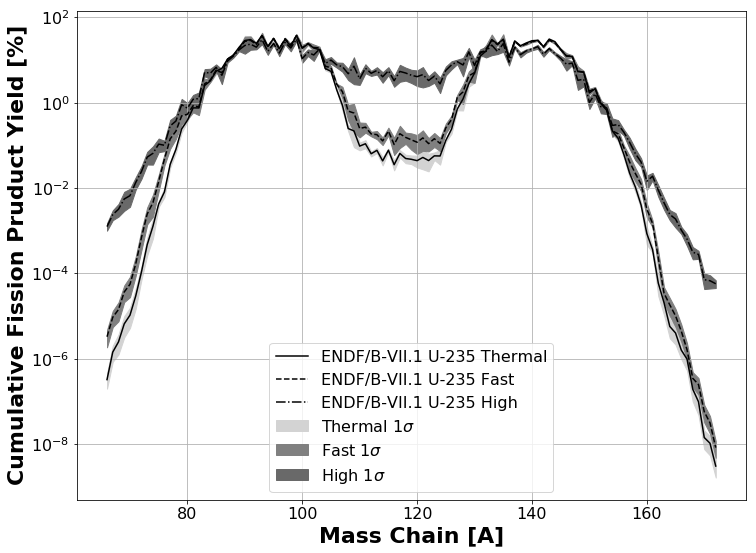
\includegraphics[width=\linewidth]{Figures/Chapter2/ENDF_FPs.png}
	\caption[Comparison of energy dependent U-235 cumulative fission product distributions]{Comparison of energy dependent U-235 cumulative fission product distributions from ENDF/B-VII.1 \cite{ENDF}.}
	\label{fig:U235Cumulative}	
\end{figure}

The chain yield for a particular mass chain is defined as the sum of the cumulative yields for the final decay to a stable or very long lived isotope in that mass chain\cite{Nichols2008}. The chain yield leads to the cumulative distribution accounting for branching in and out of a mass chain through neutron emission. 
An example is shown in Figure \ref{fig:89} for the A = 89 mass chain, where the stable isotope is Y-89\cite{SINGH20131}. 
The neutron deficient decay scheme has not been shown as it has negligible contribution to the fission product decay scheme. 

\begin{figure}[h!]
	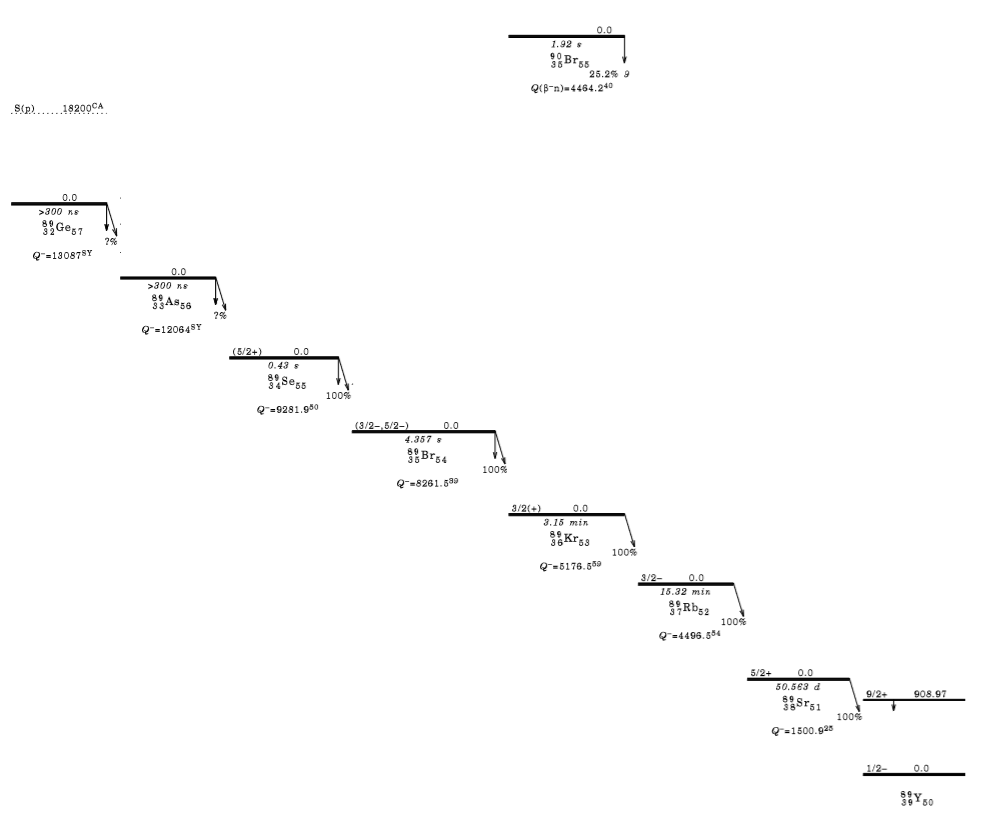
\includegraphics[width=\linewidth]{Figures/Chapter2/89MassChain.png}
	\caption[Neutron rich decay scheme for mass chain A=89.]{Neutron rich decay scheme for mass chain A=89\cite{SINGH20131}.}
	\label{fig:89}	
\end{figure}

Yields are dependent on the energy of the incident neutron and the fissioning nucleus. 
As the energy of the neutron is increased, the valley of the fission products is raised as the fission process becomes more symmetric \cite{Tonchev0}. 
Additionally, the distribution shifts to larger mass nuclides as the fissioning nucleus mass increases. 
The uncertainty in the fission product yields varies significantly; the fast fission relative uncertainty ranges from 1.6\% for mass chain 137 to 64\% for mass chain 109.   

The radioactive emissions of the final decay can be used to measure the cumulative fission product yield for an isotope. 
Some mass chains are more well-behaved for measuring the cumulative yield. For example, the $A=89$ mass chain has many decays that have very short half-lives, up to the precursor stage for the stable isotope. 


\subsection{Nagy Fits for Fission Product Yield}

Empirical relations exist to predict the fission product yield as a function of energy given sufficient yield measurement data. 
Nagy fits the fission product experimental data to an exponential equation 

\begin{equation} \label{eq:nagy}
Y(E_{n}) = Y_{0}e^{bE_{n}}
\end{equation}

The fitting parameters $b$ and $Y_{0}$ represent the slope of the function in logarithmic form and thermal fission yield, respectively\cite{Nagy1978}. 
The slope is the primary measure of the energy dependency of the fission product yield. 
The Nagy fit requires  modifications for first and second chance fission. 
First chance fission is dominant from up to 5.5 MeV, and second-chance fission up to 14.1 MeV\cite{Nagy1978}. 
The multi-chance fission effects are less likely in asymmetric regions have a larger impact in symmetric fission ($109 \leq A \leq 129$)\cite{Bevins}. 

It is important to note that data based phenomenological models are not perfect predictors of determining fission products a priori. 
In particular, recent publications have findings that contradict and cannot be accurately modeled with current theoretical approaches\cite{Tonchev0}. 
In general, there are large uncertainties in the predictive power of calculating energy dependent fission product yields. 
%A traditional method of determining fission neutron  product production is the Madland-Nix method, or some variant of, produced at Los Alamos National Laboratory (LANL)\cite{Randrup2012}. 
% The Madland-Nix method has some simplifying assumptions that allow for analytical analysis. An example simplification is that the fission product production is independent of neutron multiplicity in some variants. 

\section{Nuclear Data}

\subsection{Nuclear Data Libraries}

\ Nuclear data relevant to neutrons has been collected for the better part of the last century. 
The experimental nuclear data is collected and published in types of evaluated data files. 
There are many versions of evaluated nuclear data, which all aim to characterize the relevant physics backed by experimental results. 
For example, the U.S. nuclear data file is the Evaluated Nuclear Data File (ENDF). 
Other nations or organizations also have independent evaluations of the available nuclear data. 
Examples of other nuclear data libraries are the Russian National Library of Nuclear Data (ROSFOND), the European Joint Evaluated Fission and Fusion (JEFF) Nuclear Data Library, and the International Reactor Dosimetry and Fusion File (IRDFF).
The various evaluated libraries available have different regions of application. 
Figure \ref{fig:RxnComp} shows the evaluation of Au-197 (n,2n) for various libraries. 
In some cases, the library evaluation can be drastically different. 
However, sometimes the libraries are drawing from the same data and models, which can be noted by the overlapping evaluations. 

\begin{figure}[ht]
	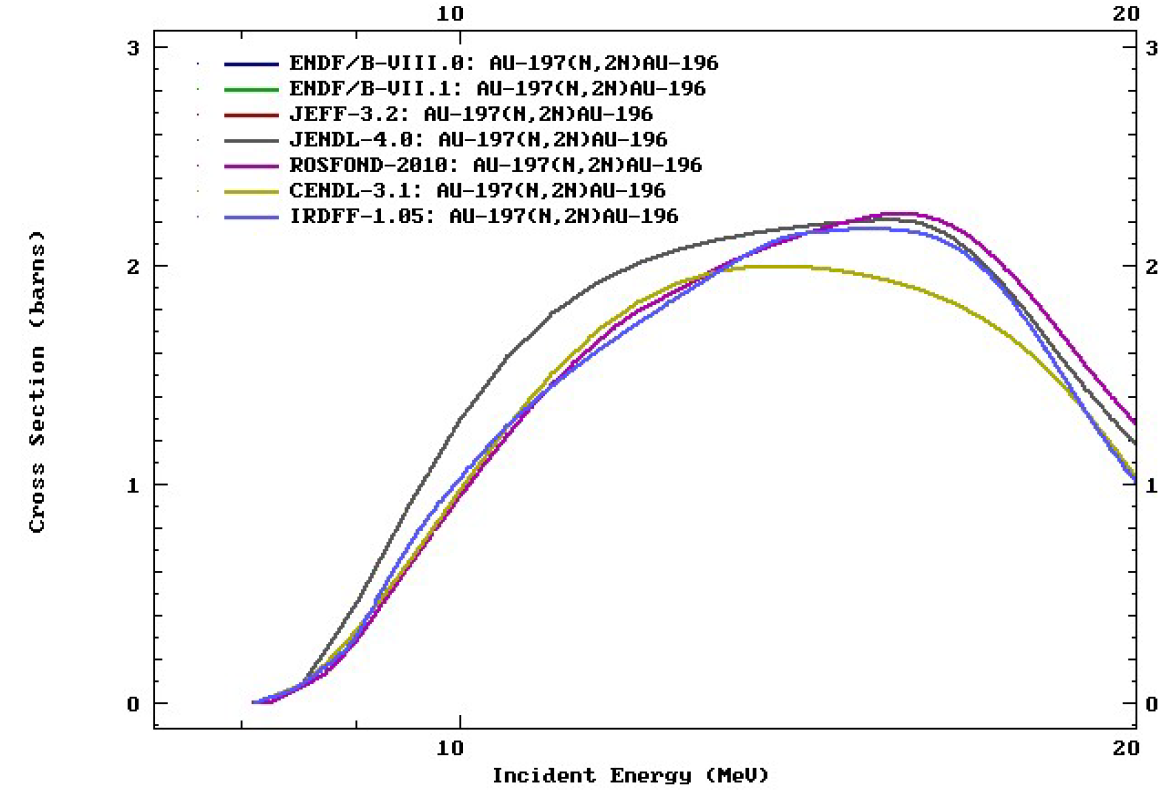
\includegraphics[width=\linewidth]{Figures/Chapter2/RxnComp.png}
	\caption[Comparison of various library evaluations of the Au-197 (n,2n) cross-section.]{Comparison of various library evaluations of the Au-197 (n,2n) cross-section \cite{ENDF}.}
	\label{fig:RxnComp}
\end{figure}

\
\ The process from which nuclear data is created varies. ENDF relies on evaluations of data based on experimental quality, statistics, and theoretical basis to fill in the areas where no experimental data exists \cite{Brown2015}. ENDF contains the underlying nuclear data (cross-sections, angular distributions, half-lives, ect.) that can be used in simulations. The experimental data that feeds into ENDF is contained in EXchange FORmat (EXFOR), where the experiment uncertainty, if available, is tracked. A large portion of these libraries are produced with reaction models. Experiments with sub-electron-volt neutron energy resolution are not feasible at the present time, so the nuclear data evaluators need models to fill in the gaps.   

\ Benchmarking the evaluated nuclear data is done primarily through testing of integral results, such as the effective neutron gain to loss ratio ($k_{eff}$) of a critical assembly \cite{Brown2015}. These integral measurements provide a more accessible measurement that can be done with high precision and accuracy, which are used to validate the microscopic nuclear data. Criticality experiments can generally be as precise as a relative error of 0.01\%\cite{Brown2015}. The use of integral benchmark experiments is important for comparing the net result of the nuclear data; however, there are uncertainties and correlations in the independent reactions that combine to create the integral results. 

\ It is important to note that some experiments, such as gamma spectroscopy, have larger uncertainty by orders of magnitude. An interesting note is that nuclear data values and uncertainty do not always decrease in relative error over time. One example is the increase in uncertainty in the neutrons released per thermal fission of U-235, which increased from 0.311\% to 0.385\% between ENDF/B-VII.0 to VII.1 \cite{Bostelmann2017}. Another example demonstrating the nuclear data problem is that He-6 half-life has changed by approximately 5\% with large increases in the relative error over the last 50 years\cite{he6}. A sub-second half-life is difficult to measure in experimental facilities. The process of creating nuclear data for application starts with experiment and theory, which is used as an evaluated library. The library is iterated on with validation experiments, applications, studies, and integral benchmarks to increase the base of the nuclear data\cite{Brown2015}. The majority of accurate measurements were performed for nuclear reactor studies, which limits accessibility to reliable data for different applications. As a consequence of this, ENDF only contains fission production data at thermal, fast (0.5 MeV), and high energy (14 MeV). There are multiple sources of nuclear data available to help alleviate this issue. 

\ The International Atomic Energy Agency provides (IAEA) provides data for the IRDFF library which contains benchmarked neutron dosimetry reactions\cite{IRDFF}. This library is noted because it is used in the PNNL STAYSL code system, which will be discussed later. The IRDFF v.1.05 library contains ``state-of-the-art" covariance information and has continuous improvement through testing and integral experiments \cite{Greenwood2017}. 

\ The IRDFF library is also convenient in the fact that some of the reactions include feed through from fast decaying excited states to metastable states. An example of this is for the In-116m1, which was shown in Figure \ref{fig:In116Rxn}. The first metastable state at 127 keV (spin parity $J^{\pi} = 5^{+}$) has a half-life of 54 minutes, which makes it a good candidate reaction for foil activation\cite{Zolotarev2013}. The IRDFF v1.05 library contains reaction data which includes the decay of the second metastable state into In-116m1. In-116m2 decays to In-116m1 with a 2 second half-life. Under standard measurement conditions, all of the In-116m2 will decay, thus contributing to the effective activity seen by the first metastable state. 

\subsection{Nuclear Data Covariance}

\ Covariance arises in nuclear related experiments when one process impacts another. 
Nuclear data covariance is not standard to experimental analysis and many times errors are attributed to model fidelity, measurement, or setup problems when nuclear data covariance might have been the root cause. %cite?
For example, in many nuclear decay processes, the covariance is unity because the decays happen in a series. 
However, covariance can occur if there is branching from a radioactive state. 
Covariance is defined with the expectation values, $<X>$, and mean value ($\mu$)
% The expectation values with the spaces don't look great. No sure how to fix though.
 
\begin{equation} \label{eq:Cov1}
      cov(X,Y) = \left\langle  XY \right\rangle-\mu_{X}\mu_{Y}, 
\end{equation}

\noindent and the covariance of an observable compared to itself reduces to the variance 

\begin{equation} \label{eq:Cov2}
      cov(X,X) = \left\langle  X^{2} \right\rangle-\left\langle  X \right\rangle^{2} = \sigma_{X}^{2}.
\end{equation}

\ Nuclear data often stores the correlation matrix using a group structure, as shown in Figure \ref{fig:coor}, instead of the covariance matrix. 
The correlation matrix combined with the uncertainty in the nuclear data is equivalent to the covariance matrix. 
The diagonal of the correlation matrix is one, so the diagonal of the covariance matrix is the variance for the group.   

\begin{figure}[h]
	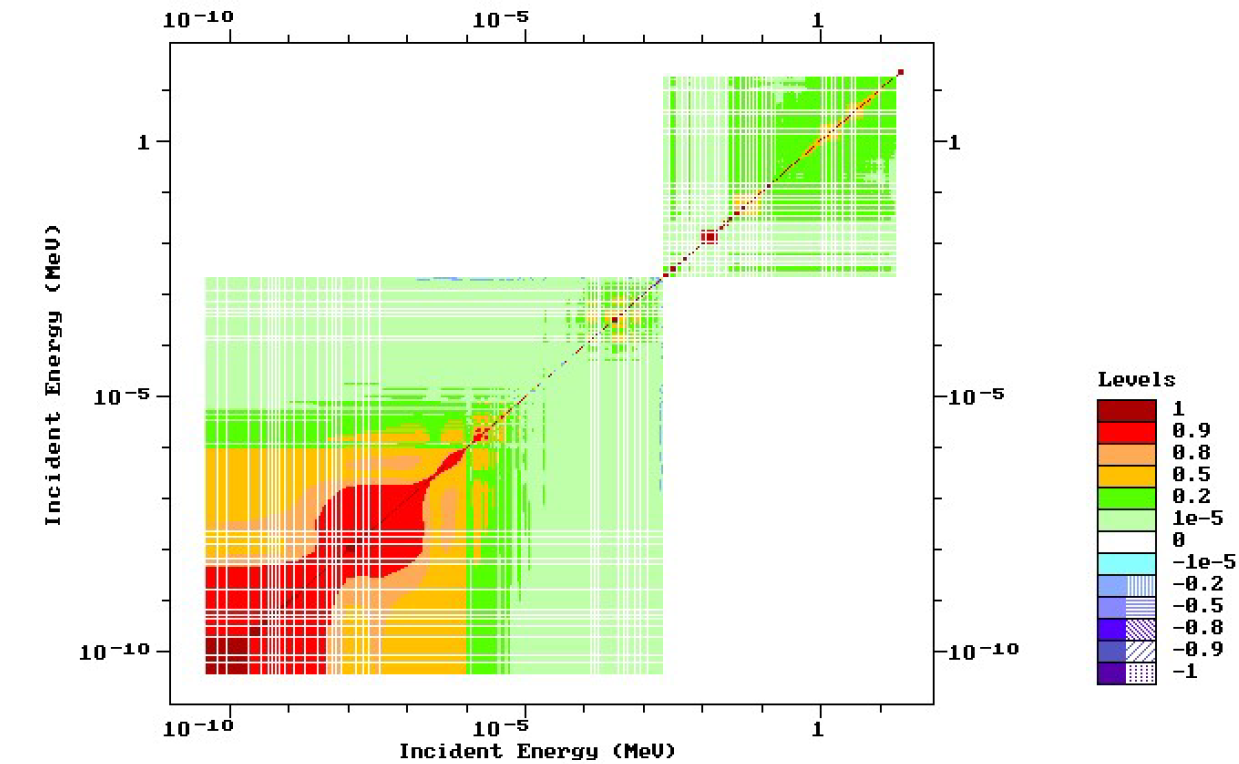
\includegraphics[width=\linewidth]{Figures/Chapter2/U235_nf_coor.png}
	\caption[$\mathrm{^{235}U}$ (n,f) correlation matrix.]{$\mathrm{^{235}U}$ (n,f) correlation matrix\cite{ENDF}.}
	\label{fig:coor}
\end{figure}

\ The most straightforward quantity to the covariance matrix is the variance across the diagonal. 
Integral experiments are extremely dependent on the underlying reactions that make up the net result. 
Therefore, there are generally larger variances in the the reactions that are part of the total cross-section. 
Figure \ref{fig:U235rel} displays the relative uncertainty of the $\mathrm{^{235}U}$ (n,f) cross-section compared to the total. 
Figure \ref{fig:Bi209rel} displays the total cross-section of $\mathrm{^{209}Bi}$ to the (n,2n) reaction. 

\begin{figure}[!]
	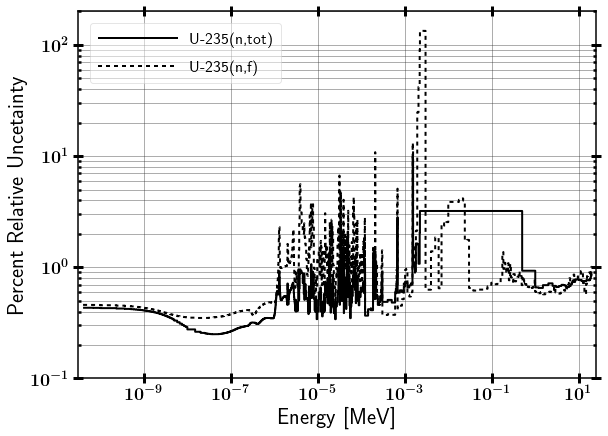
\includegraphics[width=0.9\linewidth]{Figures/Chapter2/U235_RelUncert.png}
	\caption[U-235 (n,f) compared to U-235(n,tot) cross-seciton uncertainties ]{$\mathrm{^{235}U}$ (n,f) compared to $\mathrm{^{235}U}$ (n,tot) cross-seciton uncertainties \cite{ENDF}.}
	\label{fig:U235rel}
	\vskip 0.5cm
	\includegraphics[width=0.9\linewidth]{Figures/Chapter2/Bi_209_RelUncert.png}
	\caption[Bi-209 (n,2n) compared to Bi-209 (n,tot) cross-seciton uncertainties]{$\mathrm{^{209}Bi}$ (n,2n) compared to $\mathrm{^{209}Bi}$ (n,tot) cross-seciton uncertainties \cite{ENDF}.}
	\label{fig:Bi209rel}
\end{figure}

\ The uncertainty in $\mathrm{^{235}U}$ (n,f)  and $\mathrm{^{209}Bi}$ highlight a couple key attributes relevant to nuclear data. 
First, the component reactions that make up the integral cross-section almost always have a higher relative uncertainty because integral, total cross-section experiments can more accurately be measured through attenuation of a ``beam" of neutrons. 
The underlying reactions are generally more difficult to characterize. 
The characterization is also dependent on source energy availability, which is not very broad for neutrons. 
Second, the $\mathrm{^{235}U}$ (n,f) relative uncertainty near 2.2 keV is 133.6\%, which implies that the cross-section must go negative to produce the total total result in some circumstances. 
This is obviously non-physical; however, it gives scope to the magnitude of uncertainty of the underlying cross-sections over difficult experimental energy ranges. 
Next, the $\mathrm{^{235}U}$ reactions are more thoroughly studied as compared to $\mathrm{^{209}Bi}$. 
Over the the majority of the energy range, $\mathrm{^{235}U}$ is below one percent relative error, largely driven down by thermal nuclear reactor experiments, while $\mathrm{^{209}Bi}$ has a larger error around five percent. 
Finally, areas where the cross-sections are low have representative larger relative errors, which is presented near the threshold of the $\mathrm{^{209}Bi}$ (n,2n) reaction. 

\section{Monte Carlo Neutron Transport}

\ Monte Carlo (MC) methods for neutron transport leverage pseudo-random sampling, the nuclear data, and material specifications to build up a simulation of the particles \cite{Luciano2012a}. 
Neutrons are tracked in seven-dimensional space as a function of position, direction, and energy. 
Neutron interactions are sampled with probability distribution functions (PDFs) for aspects such as path length traveled and interaction type \cite{Lewis1984}. 

\ An objective of a neutron transport calculation is to determine the behavior of particles with in the system. 
This can be captured with the scalar flux, $\bar{\phi_V}$, defined as

\begin{equation} \label{eq:flux}
\bar{\phi_V} = \frac{1}{V}\int_V dV \int_t dt \int_E dE\: \phi(\vec{r}, E,t),
\end{equation}

\noindent where  $\bar{\phi_V}$ is given as a funtion of energy, $E$, position, $\vec{r}$, and time, $t$. The scalar flux is averaged over this phase space for some discretization and averaged over a volumetric region. Monte Carlo methods approximate the scalar flux with either track length or collision estimates \cite{Lewis1984}. The track length estimator is 

\begin{equation} \label{eq:track}
\bar{\phi_V}  = \frac{W \: T_l}{V \: N},
\end{equation}

\noindent where the path length score for the flux based on the length traveled ($T_{l}$). The scalar flux is normalized by the particle weight (W), cell volume (V), and number of histories sampled (N).

\ Statistics often drive the uncertainty in a MC simulation as systematic uncertainties are generally not considered due to computational costs. 
The ``true" mean value, $\mu$, of a response PDF is the expectation value, $E(x)$, which is estimated with a sample mean, $\bar{x}$. 
The sample mean approaches the real mean as the number of samples, $N$, goes to infinity. 

\begin{equation} \label{eq:sampmean}
\bar{x} = \frac{1}{N}\sum_{i=1}^N x_i 
\end{equation}

\ The Central Limit Theorem governs the results of Monte Carlo methods and states that for large $N$, the mean of sampled $x_i$ follows a Normal distribution. 
The uncertainty is based on the spread of the results. 

\ The variance of the mean, ($S_{\bar{x}}^2$), is based on the sample variance, ($S_x^2$), 

\begin{equation} \label{eq:sampvar}
S_{\bar{x}}^2 = \frac{S_x^2}{N}
\end{equation}

\noindent where $S_x^2$ is defined as 

\begin{equation} \label{eq:sampvar1}
S_x^2 = \frac{1}{N-1}\sum_{i=1}^N (x_i - \bar{x})^2.
\end{equation}

Therefore, the uncertainty in the results decreases with $\sqrt{N}$. 
The precision of the result can be improved with more histories, shrinking the spread in $x_i$. 
However, the accuracy cannot be improved. 
Accuracy is impacted by systematic errors. 
The net result provides a 1$\sigma$ confidence bound ($\sim$68\% of values lie within 1 standard deviation of the mean). 

\section{Foil Activation}

\subsection{Foil Activation Theory}

Foil activation is a method of characterizing an incident neutron flux through unfolding the response of the foils using the energy dependent nuclear reaction channels in the foil. 
Activation experiments are essential for testing that requires small geometry to fit in the apparatus or in situations where electronics equipment for higher fidelity measuring techniques will be damaged. 

The foils intended for activation produce radioactive isotopes during the course of irradiation. 
The production rate of radioactive isotopes is negated by radioactive decay processes, which place an upper limit on the radioactivity of a foil \cite{Knoll}. 
The saturated activity ($A_{\infty}$) is equivalent to the reaction rate ($R$), which is a function of the energy dependent flux ($\phi$), the macroscopic reaction activation cross-section ($\Sigma(E)_{act}$), and the volume of  the foil ($V$). The energy term (E1) is zero in many cases; however, threshold reactions require the incident neutron to be of higher energy to enable the reaction channel. The saturated activity, ($A_{\infty}$), for a given reaction is given by:   

\begin{equation} \label{eq:InfReactionRate}
A_{\infty} = R = \int_{E1}^{E2} \phi(E) \Sigma(E) _{act} V 
\end{equation}

A correction needs to be made in cases where the activation is not sufficient 
to fully saturate the foil. At six half-lives, a foil will have reached 
approximately 98\% of its saturation activity, neglecting spatial and energy 
self-shielding effects \cite{Knoll}. The activation of the foil for a given irradiation time ($t_{i})$ is given as a function of the decay 
constant: 

\begin{equation} \label{eq:ReactionRate}
A_{0} = A_{\infty}(1-e^{-\lambda t_{i}}) 
\end{equation}

Experimental measurements also can be corrected to deduce the original activity of the foil, immediately after irradiation. The measured counts, $C$, is reduced by the background counts, $B$. A corrects for the radioactive decay for the time between the end of irradiation and the start of counting ($t_{d}$). A similar correction factor based on the count time, $t_{c}$ provides a correction for radioactive decay during counting. Additionally, the detector efficiency for the given gamma-ray energy, $\epsilon$, and relative gamma intensity, $I_{\gamma}$, must be taken into account. The gamma intensity may also include a branching ratio if applicable to the decay mechanism. All corrections included, less self-shielding effects, provide a formulation for converting counts to post-irradiation activity as:  

\begin{equation} \label{eq:MeasActivity}
A_{0} = \frac{\lambda (C-B) e^{\lambda t_{d}}}{\epsilon (1-e^{-\lambda 
t_{c}})I_{\gamma}}
\end{equation}

The formula can be simplified in the limit of irradiation times much less that 
the half-life of the activation products. In this case, the reaction rate is 
much larger than the decay from radiation, so the rate of production of the 
radioisotope is driven only by the reaction rate. The neutron pulse length at the NIF is on the order of shakes, so this approximation can be made for the foil activation. The time integrated flux, or neutron fluence ($\Phi$), can be used to determine the total reactions, ($R_{total}$),
over an irradiation period, given by:

\begin{equation} \label{eq:NIFrxnRate}
 R_{total} = \int_{E1}^{E2} \Phi(E) \Sigma(E) _{act} V \:dE 
\end{equation}

\subsection{Selection of Experimental Foils}
% Update this section with feedback from NENG 612 paper
\ The foils selected must meet several requirements depending on the 
experiment. The method of foil activation has been studied in-depth in the 
nuclear sciences and engineering community. A list of the various 
requirements that are of importance for a neutron activation foil experiment 
with energies in the range of thermal to approximately 20 MeV is summarized\cite{Knoll,Luciano2012a,Kuijpers1977}.

\begin{itemize}
	\item The reaction neutron cross-section is extremely important for foil 
	activation, and there are a few key parameters that should be considered. 
	First, the magnitude of the cross-section determines the 
	reaction rate of the product nuclides. A large cross-section allows for 
	more activation, and therefore, better results when analyzing the activation 
	foils. Second, the uniqueness of the cross-section shape is used to unfold 
	the incident neutron energy spectrum. An (n,$\gamma$) cross-section may 
	peak 
	in a particular region, which is essential to providing information of the 
	neutron flux in that energy region. Alternatively, a threshold reaction, 
	such as an (n,2n), is important for providing information of the flux at 
	higher energies. Third, the selected foils for an experiment should cover  
	the entire energy range of the incident neutron flux. 
    
    \item The cross-section must be well characterized with low uncertainty over the neutron energy range of interest.   
    
    \item The decay constant of the product nuclides is important. The 
    half-lives applicable for a particular experiment depend on the time 
    post-irradiation that the foils can be counted. A long lived radioisotope 
    will be available for counting for longer times, but the activity will be reduced due to the lower decay constant. The opposite being true for short 
    half-lives. A half-life on the order of an hour to a few years is in the 
    right direction; however, the half-life must also be balanced with the 
    production of the radioisotope to understand the entire picture. 
    
    \item The elemental and chemical purity of the activation foil should be 
    well known. An unknown composition foil will likely cause erroneous 
    results. 
    
    \item Interfering reaction channels and decay emissions should be avoided. 
    An example of this is natural copper, which has multiple 511 keV emissions 
    from different reaction channels. It is difficult to distinguish these 
    gamma-rays to determine activation in counting. Similar problems arise in 
    multi-isotope materials that have multiple reactions producing the same 
    nuclide. For example, a Cadmium-106 (n,$\gamma$) reaction produces the same 
    isotope as a Cadmium-108 (n,2n) reaction. 

    \item The activation foil should be optically thin to not cause 
    perturbations of the neutron flux. An additional benefit of relatively thin 
    foils is that the gamma-ray emissions are not significantly attenuated 
    through self-shielding. The neutron flux should ideally also not be 
    changing substantially over the foil region. In general adding additional foils helps to improve the unfolding 
    results, as long as the entire foil set remains optically thin \cite{Vagena2018b}. 

    \item The decay nature of the product nuclide should be a gamma-ray 
    emitter. Gamma-ray detection can provide fine energy resolution to 
    determine activation. The discrete gamma-ray emissions provide a means of 
    determining the source and magnitude of the the foil activation. The energy 
    of the gamma is also of importance. Semiconductor detection methods have a 
    peak intrinsic efficiency near 100 keV with some variance depending on if 
    the semiconductor is p-type or n-type. Beta spectroscopy is also  a potential option that will be considered; however, the resolution is not as good as gamma spectroscopy.  
   
\end{itemize}


\section{Neutron Energy Spectrum Unfolding}

Foil activation experiments are a well established method for determining an 
incident neutron energy spectrum. The foils are activated under a nearly 
equivalent neutron flux, which serves to activate the foil samples through 
nuclear reaction channels, each of the which has a unique response 
function with respect to the neutron flux. The nuclear data and activities of 
the foils can be used to unfold the incident neutron energy spectrum.
The activated foil 
production is just the group-wise energy multiplication of the reaction 
cross-section with the neutron flux. 

The activated foil production is just the group-wise energy multiplication of the reaction cross-section with the neutron flux, but solving for the inverse problem for the neutron flux is generally seen as ``ill-posed" \cite{Vagena2018b}. 
In an ideal situation, the number of foils, $i$, would be selected based on the number of energy groups, $j$ required, and the problem would be formulated as \cite{Vagena2018b, Luciano2012a}  

\begin{equation} \label{eq:BadWaytoGetFlux}
    A_{i}= \sum_{j=1}^{N} \; \Sigma_{i}(E_{j}) \;\Phi(E_{j}) \;V,\;\; 
    i=1..m 
\end{equation}

\noindent In practice, this formulation of the unfolding problem is not used as it often provides nonphysical results.
The issue is caused by the varying shapes of reaction cross-sections, which create a poorly constructed matrix and a limit on the number of foils that can be used at a time to prevent changing the neutron flux. 
There are many methods that aim to provide solutions to the generally degenerate neutron spectrum. 

A few examples of studied methods of unfolding matrix inversion, least-squares spectral adjustment, and stochastic algorithms\cite{Reginatto2010}. 
Direct matrix inversion was previously discussed in the setup of the unfolding problem. 
Matrix inversion can lead to non-physical results, such as negative fluxes \cite{Reginatto2010}. 
Stochastic methods rely on random sampling to derive a best-fit or average over a group of reasonably well-fitting spectra\cite{Reginatto2010}. 
The least-squares method minimizes the chi-square based on a guess spectrum, activation information, and nuclear data \cite{Perey1977}.
The least-squares method is also known as spectral adjustment and can incorporate more information, most notably the underlying nuclear data, into the determination of the resultant spectrum \cite{Perey1977}.  

The general formulation of the least-squares method is derived from minimizing the activation results to the nuclear data and input spectrum\cite{Perey1977}. 
The chi-square ($\chi^{2}$) is given as per degrees of freedom ($DOF$) as a function of of the uncertainty, activation rates, nuclear data, and measured results. 
The chi-square formulation of the least-squares approach can be reduced if there is no time dependency of the neutron flux as

\begin{equation} \label{eq:LeastSq}
\dfrac{\chi^2}{DOF}= \dfrac{1}{DOF}\sum_{i=1}^{m} \; \dfrac{(\sum_{j=1}^{N} \Sigma_{i}(E_{j}) \;\Phi(E_{j})-\dfrac{A_{i}}{V_{Foil}})^{2}}{\sigma_{i}^{2}} \,\;\; .
\end{equation}

Providing an initial spectrum is generally required for the unfolding methods. 
The activities produced for the foils is often highly degenerate, where an infinite amount of spectra could provide the same end-point. 
The initial spectrum allows for the insertion of more physics based results to have an impact on the overall result. 
For neutron spectra, an initial guess spectrum is often created with a particle transport code or a deterministic solution. 
Alternatively, an initial spectrum could be selected from published results, where in some applications provide similar results\cite{VegaCarrillo2002}. 

\ Several formulations of the $\chi^{2}$ statistic exist. STAYSL utilizes activity information, $A^{\circ}$, a neutron flux and nuclear data matrix, P, and covariance matrices. STAYSL incorporates covariance information, $N_{P}$, which is the covariance matrix from the flux and nuclear data. The activity covariance is a matrix given by $N_{A^{\circ}}$. STAYSL minimizes the $\chi^{2}$ based on the activity information, $\bar{A}$, and neutron flux and nuclear data parameters, $\bar{P}$. The $\chi^{2}$ statistic utilzied in STAYSL is given by \cite{Perey1977}. 
	
\begin{equation} \label{eq:LeastSqSTAYSL}
\chi^{2} = \begin{bmatrix}
P-\bar{P} \\
A^{\circ}-\bar{A}    
\end{bmatrix}^{\dagger}
\space 
\bullet
\space 
\begin{bmatrix}
N_{P}  &  0      \\
0  &  N_{A^{\circ}}     
\end{bmatrix}^{-1}
\space
\bullet
\space
\begin{bmatrix}
P-\bar{P} \\
A^{\circ}-\bar{A}    
\end{bmatrix}
\end{equation} 


 
